\chapter{Linear systems}
\label{ch:systems}

\chapquote{The property of the straight line as being the shortest connection between two points can be transferred to curved surfaces\ldots; on the surface of the sphere the great circles play the role of the shortest line of connection\ldots. Yet\ldots\ all great circles of the sphere intersect and therefore there are no parallels among these ``straight lines''.}{Hans Reichenbach, German philosopher of science}

Many important natural and manmade phenomena can be represented using mathematical functions. We may have to work quite hard to figure out the best way to ``mathematize'' a real-world context, but once we do we can very often learn something about the real-world from studying the our mathematical representation.

In this chapter we will learn a set of techniques for understanding how functions interact. We will continue our focus on linear functions, though many of the ideas can be applied to other situations. In the last section, we'll explore some classic applications of the tools and techniques that we learn in the earlier sections.

%%%%%%%%%%%%%%%%%%%%%%%%%%%%%%%%%%%%%%%%%%%%%%%%%%
\section{Mathematical modeling}
\label{sec:sysintro}

Mathematics has many applications to the sciences, medicine, business, and economics. Often, though, we have to ``translate'' some problem in the real world so that it can be interpreted mathematically. It is usually necessary to break down the situation into a set of variables and equations, then look at them all together and see how they interact with each other. Doing this is called \inlinedef{mathematical modeling}.
\index{mathematical modeling}

In this way we can model the financials of a business, weather patterns, transportation infrastructure, airline schedules, missile guidance systems, factory efficiency, and many other phenomena.

\begin{boxexplore}[{I} $\varheart$ {C}heeseville {Z}oo]
After YeardleighCorp took over and renovated the failing Cheeseville Zoo, Yeardleigh launched a marketing campaign to announce the grand reopening. She spent \$270 on a t-shirt design. For production, she found a supplier who sold her blank cotton shirts in a variety of sizes and colors for \$3.00 per shirt, and a printer who would print the logo in full color for \$1.50 per shirt. If Yeardleigh sold the shirts for \$12.00 each, how many would she have to sell before she started to make a profit on t-shirt sales?
\end{boxexplore}

%\begin{boxexplore}[{I} $\varheart$ {Y}eardleigh{C}orp]
%Yeardleigh is a good business woman. She realizes that in order to grow her business, she must brand her corporation by selling things like t-shirts with her company logo on it. She spends \$270 on a design. Since she plans on printing a huge number of shirts, she finds a supplier who will sell her blank cotton shirts in a variety of sizes and colors for \$3.00 per shirt, and a printer who will print the logo in full color for \$1.50 per shirt. If Yeardleigh decides to sell the shirts for \$12.00 each, how many shirts must Yeardleigh sell before she can start making a profit on t-shirt sales?
%\end{boxexplore}

\kverse{Yeardleigh creates t-shirts in a marketing campaign.}

%%%%%%%%%%%%%%%%%%%%%%%%%%%%%%%%%%%%%%%%%%%%%%%%%%
\subsection{Simultaneous equations}

One approach to mathematical modeling is to model problems using multiple functions, and then exploring how those functions relate to one another. 

\begin{boxdef}[System of equations]
A set of two or more equations with the same variables is called a \gls{system of equations}. They are also sometimes called \textit{simultaneous equations}.
\end{boxdef}

%Real graphic designers charge much more than \$270. Real businesses have hundreds, thousands, even millions of variables and just as many constraints/limits. The goal is always to maximize profits and be more efficient. 

%Real graphic designers charge much more than \$270. Real businesses have hundreds, thousands, even millions of variables and just as many constraints/limits. The goal is always to maximize profits and be more efficient. You can't always just use one equation to do all of this. It is often easier to break down the situation into smaller equations and look at them all together and see how they interact with each other. Doing this is called ``modeling.'' You can model businesses, weather patterns, transportation infrastructure, airline schedules, missile guidance systems, how to run refineries in the most efficient way, etc. in this manner.

In the startup exploration, the amount of money Yeardleigh earns will depend on how many t-shirts she buys and sells. So, suppose we let $x$, the independent variable, represent the number of t-shirts. If we let $y$, the dependent variable, represent the amount of money, then we can write two equations: one that describes the how much the t-shirts cost, and another that describes how much money the t-shirts generate for the company.

Yeadrleigh earns \$12.00 for every t-shirt she sells, so one equation involved with the scenario is \[y = 12.00x \qquad\text{Yeardleigh's income equation}.\] She has already spent \$270 on her design, and every t-shirt she prints costs an additional \$4.50 (that's \$3.00 for the shirt and \$1.50 for printing). So, another equation in the scenario is \[y = 270 + 4.50x\qquad\text{Yeardleigh's cost equation}.\]

We now have to linear equations. Observe what happens when we graph these two equations on the same set of axes (\cref{fig:tshirts}). What does this graph tell us about the problem?

\begin{figure}[!htbp]
\centering
\resizeplot{0}{0}{50}{500}
\begin{tikzpicture}
	\begin{axis}[
			clip=false,
			width=0.625\linewidth,
			height=0.625\linewidth,
			axis lines = middle,
			axis line style={thick, ->, shorten >=-10pt, shorten <=-10pt},
			xlabel={\large Number of t-shirts sold},
			ylabel={\large Dollars spent/earned},
			grid=both,
			xlabel near ticks,
			minor xtick={0,5,...,50},
			ylabel near ticks,
			minor ytick={0,50,...,500},
		]
		\addplot[algcurve, ->, red, domain=0:50] (\x,4.5*x+270);
		\addplot[algcurve, ->, green!50!black, domain=0:42] (\x,12*x);
		\addplot[algpoints, black] coordinates {(36,432)};
		\draw[green!50!black] (axis cs:20,200,0)
			node[rotate=50.2]{\large$y=12.00x$};
		\draw[red] (axis cs:15,365,0)
			node[rotate=24.2]{\large$y=4.50x+270$};
		\draw (axis cs:36,432,0) node[below right]{\large$(36,432)$};
	\end{axis}
\end{tikzpicture}
\caption{Graph showing both Yeardleigh's cost and income equations.}
\label{fig:tshirts}
\end{figure}

On the graph in the figure, the red line is Yeardleigh's cost equation and the green line is Yeardleigh's income equation. The $x$-coordinate shows the independent variable (number of shirts), and the $y$-coordinate shows the dependent variable (amount of money spent or earned).

Notice that these two lines intersect (in other words: they cross over one another). Does this intersection point have any special significance?

The intersection shows that for a certain number of t-shirts, cost and income are the same. The points to the left of the intersection show where cost is greater than income, points to the right of the intersection show where income is greater than cost. So that intersection point is really important for the problem!

The coordinates of the intersection point are $(36, 432)$. So, if Yeardleigh sells 36 t-shirts, she will make 432 in income\ldots\ and it will also cost her exactly that much to produce the t-shirts. If she sells more than 36 t-shirts, she will earn more than it costs to make the shirts.

We have found Yeardleigh's \textit{break-even point}, a very important idea in economics and business. It is the point where a company's costs and income are the same. Before this point, the company will be losing money. After this point, the company will start to make a profit. In the context of our problem, Yeardleigh will make a profit on t-shirt sales only if she sells more than 36 shirts.

\subsubsection{Writing a system of equations}

When we have two (or more) equations that we want to treat as a system, we usually write them stacked vertically, and we very often add a big curly brace (usually on the left-hand side only) to show that they are meant to be considered a group. In the case of the startup exploration, we write: \[\left\{\begin{array}{l}y=12.00x\\y=4.50x+270\end{array}\right.\]

%%%%%%%%%%%%%%%%%%%%%%%%%%%%%%%%%%%%%%%%%%%%%%%%%%
\subsection{Solutions to systems}

\begin{boxexplore}[Imagining intersections]
Imagine two lines drawn in the coordinate plane. In the previous section, we saw that these lines might intersect at a single point. Is that the only possibility? Could they intersect in more than one point? Could they not intersect at all?

What about if we have three lines in the plane? Describe the ways they might (or might not) intersect.

What about a parabola and a line? What about two parabolas?
\end{boxexplore}

\addtodoitem{Visuals of the various solutions types.}

In the startup exploration, we are visualizing the possible solutions to various possible systems of equations.

\begin{boxdef}[Solution to a system of equations]
The set of all points that are common to all equations in the system. Graphically, these are the points where all of the graphs of the functions intersect. Note: a system of equations may have no solution.
\end{boxdef}

We will focus in this course on systems of two linear equations, and there are three ways in which two lines in the plane might interact:
\begin{itemize}
\item The lines might intersect at a single point. Such a system has a unique solution.

\item The lines might be parallel and not intersect at all. In this case, the system has no solution.

\item The lines might overlap completely (that is, the ``two lines'' might actually be the same line). In this case, the system has infinitely many solutions: every point one line is also on the other line -- they're the same line!
\end{itemize}

Since we have straight lines, these are the only possibilities. For example, a system of linear equations cannot have ``exactly two soltuions''. (Can you explain why not?) Later (in Algebra 2, for instance), systems will get more complex. Then, we won't have to limit ourselves to linear equations! A system of two quadratic equations, for example, might have no solution, one solution, two solutions, or infinitely many solutions. (Can you picture how each of those might happen? Look back at some of the graphs we drew in \cref{ch:graphs} and \cref{ch:functions}.)


\subsection{Checking a solution}

Suppose we have a point that we think might be a solution to a system of equations. How can we check?

\begin{boxex}
Determine whether or not the point $(-1,5)$ is a solution to each of the given systems.
\[
\text{System A: }\twosystem{x+y=4}{x=-1}
\qquad
\text{System B: }\twosystem{y=-x+4}{y=-\tfrac{1}{5}x}
\] 

%\[
%\text{System A: }\left\{%
%\begin{array}{l}
%x+y=4\\
%x=-1
%\end{array}
%\right.
%\qquad
%\text{System B: }\left\{%
%\begin{array}{l}
%y=-x+4\\
%y=-\tfrac{1}{5}x
%\end{array}
%\right.
%\] 

To check whether the point is a solution to System A, we'll sustitute $x$ and $y$ into both equations. If the point makes both equations true, then the point is a solution to the system.

Checking System A, we have:
\[
\begin{aligned}[t]
x+y		&=4\\
(-1)+5	&\overset{?}{=}4\\
4 		&\overset{\checkmark}{=} 4\\
\end{aligned}
\qquad\text{and}\qquad
\begin{aligned}[t]
x 	&= -1\\
-1	&\overset{\checkmark}{=}  -1
\end{aligned}
\]
The given point makes both of the equations true, so yes, the point $(-1,5)$ is a solution to System A.

Checking System B, we have:
\[
\begin{aligned}[t]
y		&=-x+4\\
5		&\overset{?}{=}-(-1)+4\\
5 		&\overset{\checkmark}{=} 5\\
\end{aligned}
\qquad\text{and}\qquad
\begin{aligned}[t]
y 	&= -\tfrac{1}{5}x\\
5	&\overset{?}{=} -\tfrac{1}{5}(-1)\\
5	&\neq \tfrac{1}{5}
\end{aligned}
\] 
The given point works for the first equation, but not for the second. To be a solution, the point has to satisfy both equations, so no, the point $(-1,5)$ is not a solution to System B.
\end{boxex}

\subsection{Writing solutions}

When we were solving equations (meaning one equation at a time) we used set notation to record our solutions. Since the solution to a system involves two numbers, we have to be mindful about how we write our answers.

Two cases are pretty straightforward. If the system has a unique point as its solution, we can write that point as the solution set. For example, the solution to System A in the previous example is $\solset{(-1,5)}$. Note that we've just enclosed the point $(-1,5)$ inside the curly braces to show that the set includes that point.

The second easy case is when a system has no solution. Then, we can use the same approach for when a single equation has no solution: $\solset{~}$ or $\mathcal{S}=\emptyset$.

The trickier case is when two lines overlap completely. We can't say that the solutions in the case are ``all real numbers'' (as we said for a single equation). In this case we say that $\solset{\text{all the points on the line }y=2x}$ or write out the sentence.\footnote{An alternative is to use set notation with a fancy notation extension. We write $\solset{(x,y) \mid x, y \in \R \text{ and } y=2x}.$ This is called \textit{set builder notation}, and it uses the vertical bar to mean ``such that''. So, this math sentence read ``$\mathcal{S}$ is the set of all points $(x,y)$ such that $x$ and $y$ are real numbers and $y=2x$.''}


\subsection{Techniques for solving linear systems}

Over the next few sections, we will study three different techniques for solving systems of linear equations. A fourth technique, which we only mention here, will be an important topic in Algebra 2.

\begin{enumerate}
\item \inlinedef{Graphing the system.} To solve a system by graphing, we graph the equations on the same set of coordinate axes and look for the intersection point. If we are lucky, we'll get ``nice'' points with integers for their coordinates. Graphing with technology works a little better, since trace functionality can give us good estimates for the coordinates if they are not integers.

\item \inlinedef{Collapsing the system by substitution.} To collapse a system is to do something algebraically that fuses two equations into one. If done correctly, we can turn two equations in two variables into one equation in one variable! One method uses the property of substitution to achieve this.

\item \inlinedef{Collapsing the system by elimination.} This is an alternative approach to collapsing a system, that is based on a mathematical structure called a matrix (although we won't go into detail about matrix operations.)

\item \inlinedef{Modeling the system as a matrix.} A \textit{matrix} (plural: matrices) is a rectangular arrangment of numbers. Matrix operations are good for solving systems with more than two variables, which we won't see in Algebra 1. We will learn much more about matrices (in general) in Algebra 2, along with a number of ways of using them to solve systems.
\end{enumerate}

The different approaches have pros and cons, and you may find that you prefer a particular approach. Generally speaking, you should solve problems using whatever techniques make the most sense to you, and some assignments will be open and allow you to choose your own method. Other assignments may ask you to use a specific technique, though, so its important to read directions carefully.

%%%%%%%%%%%%%%%%%%%%%%%%%%%%%%%%%%%%%%%%%%%%%%%%%%
\section{Solving by graphing}
\label{sec:sysgraphing}

We solved the startup exploration at the start of \cref{sec:sysintro} by graphing two equations on the same set of axes. That's the idea behind this solution technique. We graph the two lines given in our system on the same set of axes, and then we look to see how the two lines interact.

\begin{figure}
\begin{minipage}[t]{\textwidth/3}
\centering

\resizeplot{-5}{-5}{5}{5}
\begin{tikzpicture}
	\begin{axis}[standard, fullsize]
		\addplot[algcurve, blue, domain=-3.5:1.5] {2*\x+2};
		\addplot[algcurve, red, domain=-5:5] {-0.25*\x-2.5};
	\end{axis}
\end{tikzpicture}

One solution.
\end{minipage}%
%
\begin{minipage}[t]{\textwidth/3}
\centering

\resizeplot{-5}{-5}{5}{5}
\begin{tikzpicture}
	\begin{axis}[standard, fullsize]
		\addplot[algcurve, blue, domain=-3.5:1.5] {2*\x+2};
		\addplot[algcurve, red, domain=0.5:5] {2*\x-6};
	\end{axis}
\end{tikzpicture}

No solution:\\parallel lines.
\end{minipage}%
%
\begin{minipage}[t]{\textwidth/3}
\centering

\resizeplot{-5}{-5}{5}{5}
\begin{tikzpicture}
	\begin{axis}[standard, fullsize]
		\addplot[algcurve, blue, domain=-3.5:1.5] {2*\x+2};
		\addplot[algcurve, red, dashed, domain=-3.5:1.5] {2*\x+2};
	\end{axis}
\end{tikzpicture}

Infinitely many solutions:\\the two lines are the same.
\end{minipage}
\end{figure}

We graphed quite a few lines in the previous chapter, and all of those skills come into play now. When graphing by hand, it's always a good idea to use graph paper but remember that the graph itself is not the answer. The graph is the work that helps us to find the solution to the system. This means that we don't always need to create a ``high quality graph''. Of course, the graph must be of high-enough quality that you can accurately find the intersection point!

Solving by graphing can be made easier with the right technology, though technology also imposes some restrictions. If you graph using a calculator or an online graphing tool, the equation may have to be in a $y=$ form (either slope-intercept form or point-slope form). Also, technology might not help if the answers don't come out ``nice''. It may be hard to identify some rational and irrational numbers from the decimal that we get as output form the calculator!

These restrictions are avoided with the algebraic methods we will learn for solving a system (in the upcoming sections). Still, graphing will often come in handy as one good way to check our answers.

%%b. Graphing By Calculator: They have to be in function form for the graphing calculators that we have in class. The ``trace'' function is pretty useless as I expect exact answers. You should look at the table to find exact answers. On the table you will notice that the solution will show up as 1 x-value with the same y-value for the two equations.

%%\subsection{Finding an intersection point using a calculator}
%%
%%When finding an intersection point using a calculator, we may be tempted to use the \calculator{trace} function. But, \calculator{trace} can only give us a decimal approximation, and this could be a problem for some solutions. (For example, a solution that does not have whole number coordinates.)
%%
%%Using \calculator{trace} is good for approximating a solution, but then we can use an alternative way: looking at the table. Here, we can search the table for a place where \calculator{y1} and \calculator{y2} are the same for a particular value of \calculator{x}.
%%
%%For the t-shirt example, go to the \calculator{table} screen on your calculator, and scroll to where \calculator{x} is 36. You should see that both \calculator{y1} and \calculator{y2} are 432. This will be how the intersection point will show up in a table.

%%%%%%%%%%%%%%%%%%%%%%%%%%%%%%%%%%%%%%%%%%%%%%%%%%
\section{Solving by substitution}
\label{sec:syssubstitution}

\begin{boxexplore}[Ugly graphing]
Solve the following system by graphing.
\[\twosystem{y=\frac{1}{3}x-4}{y=5x-6}\]
What are the challenges that arise when solving this system graphically?
\end{boxexplore}

The challenge we uncover in the startup exploration is that the intersection point does not have integer coordinates. The $x$-coordinate is between 0 and 1, and the $y$-coordinate is between $-3$ and $-4$, but beyond that it is quite hard to find an exact intersection, even using graphing technology (since the decimal values of the intersection point are not all that ``nice'').

\resizeplot{-3}{-8}{7}{1}
\begin{center}
\begin{tikzpicture}
	\begin{axis}[standard]
		\addplot[algcurve, blue, domain=-3.5:7.25] (\x,\x/3-4);
		\draw[blue] (axis cs:4,-3,0) node[right]{\large$y=\frac{1}{3}x-4$};
		\addplot[algcurve, red, domain=-0.5:1.5] (\x,5*\x-6);
		\draw[red] (axis cs:1.5,1,0) node[right]{\large$y=5x-6$};
%		\addplot[algpoints, red] coordinates {(4,5)};
	\end{axis}
\end{tikzpicture}
\end{center}

%\begin{center}
%\begin{tikzpicture}[scale=0.75]
%		%% grid setup
%		\draw[very thin, color=gray!25] (-3,-8) grid (6,1);
%		\draw[<->,thick] (-3,0) -- (6,0);	% x-axis
%		\draw[<->,thick] (0,-8) -- (0,1);	% y-axis
%		\foreach \x in {-3,...,6}
%			\draw (\x,0.05) -- (\x,-0.05) node[below] {\footnotesize\x};
%		\foreach \y in {-8,...,1}
%			\draw (-0.05,\y) -- (0.05,\y) node[left] {\footnotesize\y};
%		%% graph
%%		\draw[red] (-1,5) node[left] {\large$y=\umin3(x+1)+7$};
%%		\draw[red] (-1,4) node[left] {\large$y=\umin3(x-2)-2$};
%%		\draw[red] (2.5,0) -- node[above,sloped] {\large$y=2(x-4)+3$} (6,7);
%		\draw[<->, ultra thick, blue, domain=-3:6] plot (\x,\x/3-4);
%		\draw[<->, ultra thick, red, domain=-0.4:1.4] plot (\x,5*\x-6);
%\end{tikzpicture}
%\end{center}

In this section we will explore the first of two algebraic methods for solving systems of equations. These algebraic approahes will avoid the challenges demonstrated by the startup exploration. The first algebraic technique is the \textit{substitution method}.

We've been substituting numbers for variables for a long time. For example, given $f(x) = 3x + 1$, we know how to find $f(5)$ by substituting 5 for $x$ in the equation: \[f(x) = 3x+1 \quad\implies\quad f(5) = 3(5)+1 = 15 + 1 = 16\] The clever idea behind solving a system using substitution is that rather than just replacing variables with letters, we can substitute one algebraic expression for another.

\begin{boxdef}[Substitution method]
A method for solving a system of equations that involves solving one of the equations for one variable and substituting the resulting expression into a different equation.
\end{boxdef}

%Remember what it means to find the solution to a linear system: we are looking for the point they have in common. This means we are trying to find a shared point $(x,y)$. The algebraic methods collapse the two equations in two variables into one equation in one variable. Let's see some examples.

\begin{boxex}
Solve the following system using substitution.
\[
\left\{%
\begin{array}{l}
y=3x\\
y=2x-4
\end{array}
\right.
\] 

\exsoln\ We are looking for a point where the two equations have the same $x$ value and the same $y$ value. So, let's assume that the $y$'s in these two equations  are equal. If the two $y$'s are equal, then it means ``$3x$'' is equal to ``$2x-4$'' and that is a Level 4 linear equation (one with variables on both sides)!
\[\begin{aligned}
3x &= 2x -4
&& \quad\text{substitution}\\
x &= -4
&& \quad\text{SPOE: subtract $2x$ from both sides}\\
\end{aligned}\]
So, if the two $y$ values are equal, as we assumed they were, then it must be that $x=-4$. We just found the $x$-coordinate of the intersection point! How can we find the $y$-coordinate?

Notice that the first equation says $y = 3x$. So, if $x=-4$, it must be that $y = 3x = 3(-4) = -12$. So, the solution to the system is the point $(-4, -12)$. Or we can write $\solset{(-4,-12)}$.

To check out work, we can either graph the system, or plug the $x$ and $y$ values into the other equation to verify that equality holds.
\[\begin{aligned}
y &= 2x -4
&& \quad\text{the second equation we were given}\\
-12 &\overset{?}{=} 2(-4)-4
&& \quad\text{substitute our proposed solution}\\
-12 &\overset{?}{=} -8-4
&& \quad\text{simplify right-hand side}\\
-12 &\overset{\checkmark}{=} -12
&& \quad\text{}\\
\end{aligned}\]
\end{boxex}

When we assume that the two $y$'s were equal -- as they must be if we have found a solution to the system -- then substitution means that we can replace one $y$ with the other.

We can carry this out for the problem in the startup exploration. Since we have two equations in $y=$ format, and since any point that satisfies the system has a $y$-coordinate that satisfies both equations, we can set the equations equal to one another:
\[\begin{aligned}
\frac{1}{3}x - 4 &= 5x - 6
&& \quad\text{substitution}\\[1ex]
2 &= \frac{14}{3}x
&& \quad\text{SPOE: variable terms to the right, constants to the left}\\[1ex]
\frac{6}{14} &= x
&& \quad\text{MPOE}\\[1ex]
\frac{3}{7} &= x
&& \quad\text{simplify the fraction}
\end{aligned}\]
Aha! Even though this $x$-value is inconvenient to graph by hand (since it's not an integer) or using technology (since it's not a very tidy decimal)\ldots\ it emerges with no trouble using substitution.

To find the $y$-coordinate, we use our newly-discovered $x$-coordinate and one of the two original equations. Why not pick the second equation to minimize the fractions?
\[\begin{aligned}
y &= 5x - 6
&& \quad\text{the second equation}\\[1ex]
y &= 5\left(\frac{3}{7}\right)-6
&& \quad\text{substitute in our new $x$-value}\\[1ex]
y &= \frac{15}{7} - 6
&& \quad\text{multiply fractions}\\[1ex]
y &= \frac{15}{7}-\frac{42}{7}
&& \quad\text{write with a common denominator}\\[1ex]
y &= \frac{-27}{7}
&& \quad\text{simplify the fraction}
\end{aligned}\]
To check our work, we can substitute our candidate values for $x$ and $y$ back into the first equation. Note that since we used the second equation already to figure out the answer, we use the first equation to check it.
\[\begin{aligned}
y &= \frac{1}{3}x - 4
&& \quad\text{the first equation}\\[1ex]
\frac{-27}{7} &\overset{?}{=} \frac{1}{3}\left(\frac{3}{7}\right)-4
&& \quad\text{substitute in our candidate solution}\\[1ex]
\frac{-27}{7} &\overset{?}{=} \frac{3}{21}-4
&& \quad\text{multiply fractions}\\[1ex]
\frac{-27}{7} &\overset{?}{=} \frac{3}{21}-\frac{84}{21}
&& \quad\text{write with a common denominator}\\[1ex]
\frac{-27}{7} &\overset{?}{=} \frac{-81}{21}
&& \quad\text{subtract fractions}\\[1ex]
\frac{-27}{7} &\overset{\checkmark}{=} \frac{-27}{7}
&& \quad\text{simplify the right-hand side}
\end{aligned}\]
So, we have found our solution $\solset{\left(\frac{3}{7}, -\frac{27}{7}\right)}$.

In the two examples we have seen so far, both equations have been in $y=$ format. This is not a requirement for using substitution, as the following two examples will demonstrate.

\begin{boxex}
Solve the following system using substitution.
\[
\left\{%
\begin{array}{l}
y=3x-5\\
x-y=4
\end{array}
\right.
\] 

\exsoln\ Here, we have one equation in point-intercept form, and one equation in standard form. No problem! We simply substitute $y$ from the first equation for $y$ in the second equation. It's a good idea to use patentheses when doing the substitution: watch what happens with the negative signs in this example.
\[\begin{aligned}
x-y &= 4
&& \quad\text{start with the second equation}\\
x-(3x-5) &= 4
&& \quad\text{substitue $y$ from first equation, using parentheses}\\
x - 3x + 5 &= 4
&& \quad\text{distributive property}\\
-2x + 5 &= 4
&& \quad\text{combine like terms}\\
-2x &= -1
&& \quad\text{SPOE}\\[1ex]
x &= \frac{1}{2}
&& \quad\text{DPOE}
\end{aligned}\]
This tells us that if the $y$'s are equal, then it must be that $x=\frac{1}{2}$. To find the $y$-coordinate, we substitute the $x$ value we just found back into one of the original equations. Let's choose the second equation, which seems a bit easier:
\[\begin{aligned}
x-y &= 4
&& \quad\text{the second equation}\\[1ex]
\frac{1}{2}-y &= 4
&& \quad\text{substitue $x = \tfrac{1}{2}$, which we just computed}\\[1ex]
-y &= \frac{7}{2}
&& \quad\text{SPOE}\\
y &= -\frac{7}{2}
&& \quad\text{MPOE}\\
\end{aligned}\]
So, $\solset{\left(\frac{1}{2}, -\frac{7}{2}\right)}$. To check we can plug these values back into the other equation (the first equation, in this case, since we used the second equation to find $y$).
\[\begin{aligned}
y &= 3x-5
&& \quad\text{the first equation}\\[1ex]
-\frac{7}{2} &\overset{?}{=} 3\left(\frac{1}{2}\right)-5
&& \quad\text{substitue our proposed solution}\\[1ex]
-\frac{7}{2} &\overset{?}{=} \frac{3}{2}-5
&& \quad\text{simplify on the right-hand side}\\[1ex]
-\frac{7}{2} &\overset{?}{=} \frac{3}{2}-\frac{10}{2}
&& \quad\text{}\\[1ex]
-\frac{7}{2} &\overset{\checkmark}{=} \frac{-7}{2}
&& \quad\text{}
\end{aligned}\]
\end{boxex}

Notice that after our substitution step, we've been getting linear equations like the ones we saw in \cref{ch:equations}.

In the first example in this section, we got an equation with the variable $x$ on both sides. Recall that when equations have variables on both sides, we sometimes find that the equation had one unique solution, sometimes ``no solution'', and sometimes ``infinitely many solutions''. Do you see how these correspond to the different possible solutions to a linear system?

The key to the substitution method is that we need at least one equation to be in $x=$ or $y=$ form. What if neither equation is in this form? We can use our skills at transforming formulas to create what we want!

\begin{boxex}
Solve the system by substitution.
\[
\left\{%
\begin{array}{l}
3x-12y=15\\
x-4y=7
\end{array}
\right.
\] 

\exsoln\ We could transform either equation, but notice that there's less work to do in the second equation, since the $x$ term has coefficient 1. So, let's transform the second equation to $x=7+4y$ using APOE. Then, we can substitute that expression into the first equation.
\[\begin{aligned}
3x-12y &= 15
&& \quad\text{the first equation}\\
3(7+4y)-12y &= 15
&& \quad\text{substitute our expression for $x$}\\
21+12y-12y &= 15
&& \quad\text{distributive property on the left-hand side}\\
21 &= 15
&& \quad\text{D'oh.}\\
\end{aligned}\]
We have arrived in one of those impossible situations that tells us the equation we created has no solution. In this case, it means that the system has no solution. In other words, that these lines were parallel all along. $\mathcal{S}=\emptyset$
\end{boxex}

That was the first ``special case''. The other special case is when the two lines completely overlap. What do you suppose will happen when we solve the system that lets us know that we're in this special case?

%\begin{boxex}
%Bob's favorite second-run movie theater charges \$8 for each adult ticket and \$4 for each child ticket. The theater sold 200 tickets for a certain showing of ``Cheese Quest 3'', and collected exactly \$1304. How many of each type of ticket were sold?
%
%Let $A$ represent the number of adult tickets sold, and let $C$ represent the numbe of child tickets sold. We know that the theater sold a total of 200 tickets, so $A+C = 200$. Plus, we know how much money they made: $8A + 4C = 1304$ (eight dollars for each adult ticket, and four dollars for each child ticket, for \$1304 total).
%
%So we have the system
%\[
%\left\{%
%\begin{aligned}
%&A+C=200\\
%&8A + 4C = 1304
%\end{aligned}
%\right.
%\] 
%\end{boxex}
%
% y=2x 3 − 4x−10 2x−3 =30
%  5
% 4x −10 y = 30
% 5 4x − 4x + 30 = 30
%Solution:
%If these equations were in the same form, you will see the solution.
%30=30
%This means that we have the same line. S = any point on 4x- 10y=30

%%%%%%%%%%%%%%%%%%%%%%%%%%%%%%%%%%%%%%%%%%%%%%%%%%
\section{Solving by elimination}
\label{sec:syselimination}

\begin{boxexplore}[Ugly substitution]
Study the following system of linear equations.
\[\twosystem{4x+3y=22}{3x+5y=11}\]
What challenges would you face if you tried to solve this system by graphing? What challenges would you face if you tried to solve it by substitution?
\end{boxexplore}

The equations in the startup exploration would require quite a bit of work to graph them accurately by hand (even using our $x$- and $y$-intercept strategy for graphing lines in standard form), and we'd have to do some work so that one could be substituted into the other. The second algebraic approach to solving a system, called the \gls{elimination method}, addresses these concerns.

This technique is particularly helpful when the given equations are both in standard form. The premise behind elimination is that we use the properties of equality to, say, add two equations together. Recall that the addition property of equality says that we can add the same quantity to both sides of an equation. If we know two things are equal, we can add one thing to one side of an equation and the other thing to the other side, and still maintian equality.

\begin{boxex}
Solve the following system using elimination. \[\twosystem{y=3}{5x-y=12}\]

\exsoln\ The first equation tells us that $y$ is equal to 3. Of course, we could add $y$ to both sides of an equation\ldots\ or we could add 3 to both sides of an equation\ldots but since we know $y$ and 3 are equal we can add $y$ to one side of an equation and 3 to the other side of that equation!

In other words, we can add $y$ to the left-hand side of the second equation we are given while simultaneously add $3$ to the right-hand side. Since we know $y=3$, we know equality will be maintained! Watch what happens:
\[
\begin{aligned}
5x-y &= 12
&&\quad\text{the second equation}\\
5x-y {\color{red}+y} &=12{\color{red}+3}
&&\quad\text{add on the first equation}\\
5x &=15
&&\quad\text{combine like terms: $y$ has been eliminated!}\\
x &=3
&&\quad\text{DPOE}
\end{aligned}
\]
Having found $x$, and having $y$ given in the original system, we have $\solset{(3,3)}$.
\end{boxex}

\begin{boxdef}[Elimination method]
A method for solving a system of equations that involves adding two equations to eliminate a variable.
\end{boxdef}

The method is called ``elimination'' because it eliminates a variable.\footnote{This name is also related to a technique from the study of matrices called \textit{Gaussian elimination}.}

\begin{boxex}
Solve the following system by elimination. \[\twosystem{2x + 2y = 7}{3x - 2y = 8}\]

\exsoln\ Notice how the coefficients on the $y$ terms are opposites. If we add these two equations together, the $y$'s will be eliminated:
\[
\begin{aligned}
		&&2x + 2y	&= 7\\
+~		&&3x - 2y	&= 8\\\hline
		&&5x +0y	&= 15\\
		&&5x 		&= 15\\
		&&x 		&= 3
\end{aligned}
\]
We then substitute $x=3$ back into one of the equations to find $y = \frac{1}{2}$. So, $\solset{\left(3,\frac{1}{2}\right)}$.
\end{boxex}

The key to the elimination approach is to ``add the equations together'' so that one variable vanishes, just as the $y$ disappeared on the third in the previous example. In order to faciliatate this elimination, one or both of the equations must sometimes be multiplied by a constant before we add them (an application of MPOE).

This approach is required to handle the startup exploration. Recall, that in that problem we were asked to solve the following system by elimination.\[\twosystem{4x+3y=22}{3x+5y=11}\]
Adding these two equations won't eliminate any variables, as we have encountered in the earlier examples. But, with a few clever applicatons on MPOE, we can put ourselves into exactly the situation that we desire.

Let's make it our goal to eliminate $x$. What could we do to these equations so that we have equivalent equations but ones in which the $x$ terms have opposite coefficients?

One way (but not the only way) to accomplish this is to multiply the first equation by 3 and multiply the second equation by $-4$.
\[\begin{array}{lcl}
4x+3y=22
& \quad \xrightarrow{\quad\text{multiply through by 3}\quad}
& \quad 12x + 9y = 66
\\
3x+5y=11
& \quad \xrightarrow{\quad\text{multiply through by -4}\quad}
& \quad -12x - 20y = -44
\end{array}\]
Then, we add equations:
\[
\begin{aligned}
		&&12x + 9y		&= 66\\
+~		&&-12x - 20y	&= -44\\\hline
		&&-11y	& = 22\\
		&&y	& = -2\\
\end{aligned}
\]
Substituting $y=-2$ into the second of the original equations, we get $3x + 5(-2) = 11$. This implies that $x=7$. So, $\solset{(7,-2)}$.

%\subsection{Elimination applications}
%
%Some word problems result in equations in standard form, which are good candidates for elimination.
%
%\begin{boxex}[More mystery numbers]
%The sum of two mystery numbers is 105. The difference between them is 67. What are the two numbers?
%
%{\bfseries Partial solution:} Let $x$ represent the first number, and let $y$ represent the second number. Then, our system is:
%\[
%\left\{%
%\begin{aligned}
%&x+y = 105\\
%&x-y = 67
%\end{aligned}
%\right.
%\]
%Can you see how to take it from here?
%\end{boxex}
%
%\begin{boxex}[La tirelire]
%Fran\c{c}ois has four more dimes than quarters. He has \$6.00 total. How many of each coin does he have?
%
%{\bfseries Partial solution:} We are looking for two pieces of information, and we will write two equations to help. Let $D$ represent the number of dimes, and let $Q$ represent the number of quarters. Then, our system is:
%\[
%\left\{%
%\begin{aligned}
%&D-Q = 4\\
%&0.10D + 0.25Q = 6.00
%\end{aligned}
%\right.
%\]
%Note that our unit of money is ``dollars''. We could have used ``cents'' as the unit instead, in which case our second equation would have been $10D + 25Q = 600$.
%\end{boxex}

% % % % % % % % % % % % % % % % % % % % % % % % % % % % % % % % % % % % % % % % 
\section{Applications of systems}
\label{sec:sysapplications}

``A train leaves New York traveling south at 180 miles per hour\ldots'' If you were to read that sentence out loud in a room full of adults, you might cause some folks to start sweating and mumbling nervously to themselves. People all over the world, for generations, have been scarred by algebra word problems. But, word problems have a bad reputation.

Yes, word problems require us to ponder a bit, decipher the information we're given, and stumble around as we figure out how to proceed. But this is the process of problem solving! The algebra skills we have learned so far, along with a little determination and creativity, will serve us well as we tackle these algebra classics.

We discuss several kinds of problems below. Our general strategy is this: We'll think about the unknown quantities and relevant facts given in the problem. We'll choose variables to represent the unknowns and model the situation using equations. (Drawing pictures and making charts might help!) Then, we'll solve the equations and check to ensure our answer makes sense.

A final thought before we get started: When we encounter a new problem it can be helpful to think back over our earlier work. If we have solved a similar problem before, that can often give us ideas about a good place to start when faced with something new.

%%%%%%%%%%%%%%%%%%%%%%%%%%%%%%%%%%%%%%%%%%%%%%%%%%
\subsection{Two unknowns, two facts}

The first examples we did with substitution and elimination are of this type. We are given two unknowns and two different facts about them. The facts usually have different units, which hint at the two equations we need to write for our model.

%One way to approach this type of problem is by creating a table to organize the data.

%Yeardleigh receives a shipment of entertainment centers, the basic model weighing 30 kilograms each and the deluxe weighing 50 kilograms each, has a total weight of 880 kilograms. If there are 20 centers altogether, how many weigh 50 kilograms?

\begin{boxex}
Ticket prices at the Cheeseville Zoo were quite a bit cheaper years ago. In 1995, the zoo charged \$8 for each adult ticket and \$4 for each child ticket. On one particularly fateful day, the zoo sold 3505 tickets and collected exactly \$18,940. How many of each type of ticket were sold on that day?
\end{boxex}

The two unknowns in this problem are the number of adult tickets and the number of child tickets. The two facts are the total number of tickets sold and the total amount of money that those tickets cost. Let's use $A$ to represent the number of adult tickets and $C$ to represent the number of child tickets that were sold on this fateful day at the zoo.

%The two unknowns are the number of 30kg and 50kg centers. One set of facts has to do with quantity, the other has to do with the weight. We make these into which are rows and columns in the table. I added ``total'' columns and rows. Let's use $T$ to represent the number of 30kg centers, and $F$ to represent the number of 50kg centers.

%\begin{center}
%\begin{tabular}{r|ccc}
%				& Number of centers	& Weight per unit	& Total Weight\\\hline
%30kg centers	& $T$					& 30				& $30T$\\
%50kg centers	& $F$					& 50				& $50F$\\
%Combined		& $20$					& --				& $880$\\
%\end{tabular}
%\end{center}

%Once the table is set up, out two equations are there in the second and fourth columns.
%\[
%\left\{%
%\begin{aligned}
%&T+F=20\\
%&30T + 50F = 880
%\end{aligned}
%\right.
%\] 
%We can now solve this system using our favorite method. It looks like a good candidate for elimination! (Why?)

The fact about the total number of tickets sold tells us that one equation is
\[A+C=3505.\]
We add up the numbers of adult tickets and child tickets to find the total number of tickets that were sold. Using the other fact about the total cost of the tickets, we write the equation
\[8A+4C=18940.\]
In the second equation, the term $8A$ is the amount of money that the zoo makes from the adult tickets alone, since each adult ticket costs \$8. The term $4C$ is the total cost of all the child tickets. The sum of these two values is the total amount of money that was collected.

We can now solve this system using our favorite method. It looks like a good candidate for elimination! (Why?)

%%%%%%%%%%%%%%%%%%%%%%%%%%%%%%%%%%%%%%%%%%%%%%%%%%
\subsection{Mixture problems}

Mixture problems ask us to combine things that have different properties to create something new, with its own unique properties. Sometimes, we have to do a bit of clever thinking in order to determine information that is not directly stated in the problem. One helpful approach is to organize the given facts into a table.

%The type of mixture problem we have previously solved were very straight forward. Every number we needed was given to us directly in the problem. This is a different type of problem. There is information in the problem that is not directly stated that we will have to infer. This is where the table is really helpful.

%YeardleighCorp opens health food stores, which sell an Evil Trail Mix of raisins and roasted nuts. Raisins sell for \$3.50 per kg, and roasted nuts sell for \$4.75 per kg. How many kg of each should be mixed to make 20 kg of Evil Trail Mix worth \$4.00 per kg?

\begin{boxex}
On this fateful day at the Cheeseville Zoo, zookeeper Florence Erlenmeyer was mixing ripe bananas and roasted crickets to make her secret-recipe monkey chow.\footnote{Seven out of eight monkeys prefer Florence the zookeeper's secret-recipe monkey chow to the leading commercial brand of monkey chow, ``Primate Crunch''.} Bananas cost \$3.50 per kilogram and crickets cost \$4.75 per kilogram. How many kilograms of each ingredient did Florence mix together if the result was 20 kilograms of monkey chow worth \$4.00 per kilogram?
\end{boxex}

%Our unknowns are number of kg of raisins (let's call that $R$) and number of kg of nuts (let's call that $N$). We also have the prices of each ingredient per kg, but nothing about a total cost.

Our unknowns are the number of kiolgrams of bananas (let's call that $B$) and the number of kilograms of roasted crickets (let's call that $C$). We are given the prices of each ingredient per kilogram, but nothing about a total cost. Finding the total cost isn't that challenging though: all we have to do is multiply!

\begin{center}
\begin{tabular}{r|ccc}
				& Amount (kg)			& Unit price (\$)			& Total price (\$)\\\hline
Bananas			& $B$					& 3.50				& $3.50B$\\
Crickets			& $C$					& 4.75				& $4.75C$\\
Mixture			& 20					& 4.00				& 80\\
\end{tabular}
\end{center}

%\begin{center}
%\begin{tabular}{r|ccc}
%				& Amount (kg)			& Unit price			& Total price\\\hline
%Raisins			& $R$					& 3.50				& $3.50R$\\
%Nuts			& $N$					& 4.75				& $4.75N$\\
%Mixture			& 20					& 4.00				& {\color{red} ??}\\
%\end{tabular}
%\end{center}

The last row of the table shows that if Florence the zookeeper makes 20 kg of monkey chow worth\$4.00 per kilogram, then she has $20 \cdot 4.00 = \$80.00$ worth of monkey chow. The other rows in the table are using this same multiplication even though they each include a variable.

We now have our system of equations:
\[\twosystem{B+C=20}{3.50B + 4.75C = 80}\]
Once again, this looks like a job for elimination. (Why?)

%%%%%%%%%%%%%%%%%%%%%%%%%%%%%%%%%%%%%%%%%%%%%%%%%%
\subsection{Work problems}

Very often in a work problem, a group of workers split up a job. Working on their own, it might take different workers different amounts of time to finish the job. Our task might be to figure out how long the job will take if several workers cooperate.

A helpful way to think about problems like this is to try and identify the ``work rate'' of the various participants. If it takes someone 3 days to paint an apartment, their work rate for painting is ``one third of an apartment per day''.

%Ivan can chop a cord of wood* in 4 days, and his father, Fran\c{c}ois, can chop a cord of wood in 2 days. How long will it take them to split a cord of wood if they work together? (One cord, which is a unit of measure of volume for firewood in the US and Canada, is about 128 cubic feet\ldots but that's not really important to this problem.)

\begin{boxex}
For quality assurance purposes, Florence the zookeeper preferred to buy live crickets and toast them herself. By hand she could roast a crate of live crickets in 4 hours. She had recently invested in a Toast-O-Matic\textsuperscript{TM} cricket roaster which could toast a crate of crickets in 2 hours. How long would it take to toast three crates of crickets if both Florence and the machine work simultaneously?
\end{boxex}

If we think of the ``job'' as ``toasting one crate of crickets'', then Florence's work rate is ``1 job in 4 hours'', or ``$\frac{1}{4}$ job per hour''. Similarly, the Toast-O-Matic's work rate is ``$\frac{1}{2}$ job per hour''.

The unknown in this scenario is the amount of time that it will take them to finish the job if they work together. Let's use $t$ to represent this unknown amount of time. If our two workers each work for $t$ hours, Florence will complete $\frac{1}{4}t$ jobs and the Toast-O-Matic will complete $\frac{1}{2}t$ jobs.

\begin{center}
\begin{tabular}{r|ccc}
	& Work rate		& Work time		& Jobs done\\\hline
Florence
	& $\frac{1}{4}$	& $t$			& $\frac{1}{4}t$\\
Toast-O-Matic
	& $\frac{1}{2}$	& $t$			& $\frac{1}{2}t$\\
\end{tabular}
\end{center}

We want to know how long it takes them to toast three crates of crickets. In other words, how long it takes them to complete ``3 jobs''. This gives us the equation:
\[
\frac{t}{4} + \frac{t}{2} = 3
\]
Note that when we approached the problem in this way, we get a single linear equation rather than a system!

%If we think of the ``job'' as ``chopping one cord of wood'', then Ivan's work rate is ``1 job in 4 days'', or ``$\frac{1}{4}$ job per day''. Similarly, Fran\c{c}ois's work rate is ``$\frac{1}{2}$ job per day''. When the two guys work together, they will finish the job in some amount of time. Let's call that $t$. The rows in our table are for the individual workers.
%
%\begin{center}
%\begin{tabular}{r|ccc}
%				& Work rate				& Work time			& Amount done\\\hline
%Ivan				& $\frac{1}{4}$			& $t$					& $\frac{t}{4}$\\
%Fran\c{c}ois		& $\frac{1}{2}$			& $t$					& $\frac{t}{2}$\\
%\end{tabular}
%\end{center}
%
%Together, they complete 1 whole job (they chop one whole cord of wood). This gives us the equation:
%\[
%\frac{t}{4} + \frac{t}{2} = 1
%\]

%%%%%%%%%%%%%%%%%%%%%%%%%%%%%%%%%%%%%%%%%%%%%%%%%%
\subsection{Rate, time, distance}

``Rate, time, distance'' problems (RTD for short) come in a variety of flavors. Sometimes the participants are moving in the same direction, sometimes in opposite directions. Sometimes one of the participants has a head start, other times the participants begin moving at the same moment. Sometimes the participants start in the same location, sometimes they start in different locations\ldots

These variations can combine to produce some confusing problems, but don't panic! Many times, drawing a simple picture at the start will help us to understand how the problem is set up. If there is important information that is not directly stated in the problem, a picture can help us to find it.

\begin{boxex}
Florence the zookeeper's office was 500 feet from the entrance to the Monkey Island attraction. On this fateful morning, she loaded a fresh batch of monkey chow into a wheelbarrow and began walking on the path to Monkey Island at a speed of 4 feet per second. At precisely the same moment, Captain Snuggles, the zoo's 350-pound gorilla, escaped from Monkey Island and began running toward the zookeeper along the same path at a speed of 26 feet per second. How long did it take Florence and Captain Snuggles to meet along the path?
\end{boxex}

In this problem, we have two participants who start moving at the same time but in different locations. They move toward each other (at different speeds) until they meet in the middle somewhere.

A common mistake with this type of situation is assuming that the travelers will meet at exactly the half-way point. This will not always true! In this case, for instance Captain Snuggles moves much faster than Florence the zookeeper, and so they will meet closer to Florence's end of the path.

We might represent this with a very simple drawing:
\begin{center}%{figure}
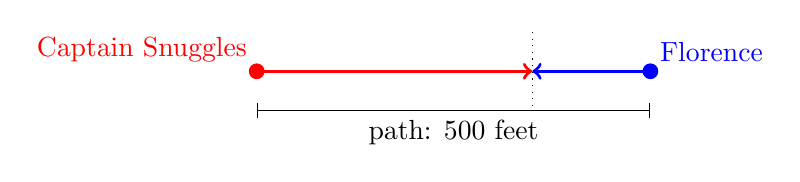
\begin{tikzpicture}
	\draw[|-|] (0,0) -- node[below]{path: 500 feet} (5,0);
	\draw[dotted] (3.5,1) -- (3.5,0);
	% gorilla
	\draw[red, very thick, ->] (0,0.5) -- (3.5,0.5);
	\fill[red] (0,0.5) circle[radius=0.1cm] node[above left]{Captain Snuggles};
	% zookeeper
	\draw[blue, very thick, ->] (5,0.5) -- (3.5,0.5);
	\fill[blue] (5,0.5) circle[radius=0.1cm] node[above right]{Florence};
\end{tikzpicture}
\end{center}%{figure}

The problem asks a question about time, so let's use $t$ to represent the time (in seconds) it takes for the two travelers to meet.

What else do we know from the problem? We have the speeds that both of the characters are moving.\footnote{We are also given the weight of the gorilla, although this is just a distraction and not important to the problem.} Florence moves at a speed of 4 feet per second, so in $t$ seconds she can travel $4t$ feet. Captain Snuggles can travel $26t$ feet in $t$ seconds. So, we can update our picture:
\begin{center}%{figure}
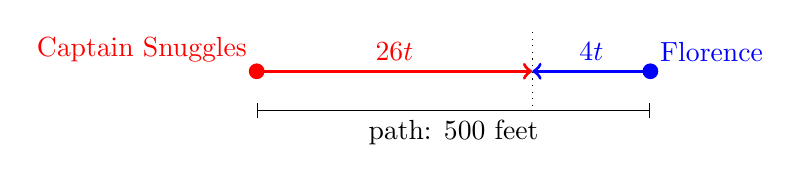
\begin{tikzpicture}
	\draw[|-|] (0,0) -- node[below]{path: 500 feet} (5,0);
	\draw[dotted] (3.5,1) -- (3.5,0);
	% gorilla
	\draw[red, very thick, ->] (0,0.5) -- node[above]{$26t$} (3.5,0.5);
	\fill[red] (0,0.5) circle[radius=0.1cm] node[above left]{Captain Snuggles};
	% zookeeper
	\draw[blue, very thick, ->] (5,0.5) -- node[above]{$4t$} (3.5,0.5);
	\fill[blue] (5,0.5) circle[radius=0.1cm] node[above right]{Florence};
\end{tikzpicture}
\end{center}%{figure}

From the drawing we can see that the combined distance that the two characters travel must be exactly 500 feet! So, we have our equation:
\[26t + 4t = 500\]
Again, we've got just a single linear equation and not a system. Who would have thought that such a complicated-looking problem would have a relatively simple mathematical representation!

%The problem is asks when Yeardleigh will pass Bob. In order to know when she will pass, we need to know when they have gone exactly the same amount of distance from the factory (this is the moment she passes him). So we'll write two distance equations, one for Bob and one for Yeardleigh, and compare them to try and figure out at what time their distances from the factories are equal.
%
%Our table columns are -- naturally enough -- rate, time, and distance. The rows deal with the people driving. The problem asks a ``when'' question, so we must be solving for time. Let's use $t$ to represent the amount of time Bob has been driving, in hours.
%
%Note that we didn't make the variable represent actual time ``on the clock''. (Why not? What challenges would that introduce into the mathematics?)
%


%%%%%%%%%%%%%%%%%%%%%%%%%%%%%%%%%%%%%%%%%%%%%%%%%%

\subsubsection{A trickier RTD problem}

\begin{boxex}
Florence the zookeeper, sadly, found herself on the business end of a hungry gorilla. Luckily, this occurred just outside the security hut, where the zoo's security squad witnessed the terrifying (but non-fatal) mauling. When they sounded the alarm, Captain Snuggles fled toward the zoo's entrance. The security squad gave chase along the same route 30 seconds later, after arming their tranquilizer guns and mounting their bicycles.

Captain Snuggles ran at 18 miles per hour. The security team cycled at 25 miles per hour, which was just fast enough: they reached the zoo entrance at the same moment as the gorilla and tranquilized him into submission. How much time elapsed between the sounding of the alarm and the tranquilizing of the gorilla? How far was the security hut from the zoo entrance?
\end{boxex}

Since the security squad started 30 seconds later, they have 30 seconds less travel time than Captain Snuggles. If we let $t$ represent the amount of time that Captain Snuggles is running (in seconds), then the security squad is chasing for $t-30$ seconds.

Even though Captain Snuggles has a head start, the security squad reaches the entrance at the same time as the gorilla because of their greater speed. So, both parties travel the same distance $d$.

Now, we have to be careful about units! The speeds in this problem are given in \emph{miles per hour}, and the time difference is given in \emph{seconds}. So, we could be careful to keep our units aligned. Let's use a little dimensional analysis (from \cref{ch:proportions}) to convert the speeds to ``feet per second''.\footnote{Alternatively, we could let $t$ represent time in minutes, and then convert the given speeds to distance \textit{per minute}. In that case, the security team would be in pursuit for $t=\frac{1}{2}$ minutes, since 30 seconds is half of one minute.}
\[
\begin{array}{r >{\displaystyle}l}
\text{Captain Snuggles:\quad}
&
\frac{18 \text{ miles}}{\text{hour}}
\cdot
\frac{5280 \text{ feet}}{\text{mile}}
\cdot
\frac{1 \text{ hour}}{3600 \text{ seconds}}
=
\frac{26.4 \text{ feet}}{\text{second}}
\\[\fracspace]
\text{Security Squad:\quad}
&
\frac{25 \text{ miles}}{\text{hour}}
\cdot
\frac{5280 \text{ feet}}{\text{mile}}
\cdot
\frac{1 \text{ hour}}{3600 \text{ seconds}}
=
\frac{36.\overline{6} \text{ feet}}{\text{second}}
\end{array}
\]

If we let $d$ represent the distance (in feet) from the security hut to the zoo entrance, then we can write an equation to describe the motion of Captain Snuggles:
\[d = 26.4t.\]
We can also model the motion of the security squad. Our formula shows both the different speed, and the fact that they start 30 seconds late:
\[d=36.\overline{6}(t-30).\]
These two equations comprise our system. Since we know that the security team and the gorilla arrive at the zoo at the same moment, we know that they travel the same amount of distance. In other words, $d$ is the same for both travelers. Substitution looks like a good choice for solving this system! (Can you explain why?)

%
%\begin{center}
%\begin{tabular}{r|ccc}
%				& Rate (mph)			& Time (hours)		& Distance (miles)\\\hline
%Bob				& 25					& $t$				& $25t$\\
%Yeardleigh		& 40					& $t - \frac{1}{2}$	& $40\left(t - \frac{1}{2}\right)$\\
%\end{tabular}
%\end{center}
%
%\[
%\left\{%
%\begin{aligned}
%&d = 25t\\
%&d = 40\left(t-\frac{1}{2}\right)
%\end{aligned}
%\right.
%\]
%
%Solving this system (substitution looks like a good choice!) will give us a value for $t$. What does that value represent? How can we use it to determine when (on the clock) Yeardleigh will pas Bob?


% % % % % % % % % % % % % % % % % % % % % % % % % % % % % % % % % % % % % % % %
\subsection{Motion in a current}

%Don't let that complicated-sounding name fool you, problems of this type are not that complicated to solve.

Have you ever tried to walk \textit{up} the \textit{down} escalator at the mall? (Be honest!) When you walk down the down elevator -- that is, when you walk in the same direction that the escalator is moving -- the motion of the escalator helps you to go faster than if you were just walking down regular stairs. On the other hand, if you try walk in the wrong direction on an escalator, the motion of the escalator will make you go slower than you would walk on regular stairs.

This is the idea of motion in a current. When you go ``with the current'' (or ``downstream'', if you're floating on a river) the current adds to your usual rate of motion. Going ``against the current'' (or ``upstream''), the current reduces your usual rate of motion.

%Bob decides to go on vacation. He takes a day trip on a river boat. The boat travels 60 km upstream (against the current) in 5 hours. The boat travels the same distance downstream in 3 hours. What is the rate of the boat in still water? What is the rate of the river's current?

\begin{boxex}
Bob and Yeardleigh were at the Cheeseville Zoo on a school field trip at the time of the mauling. When the alarm sounded, they both ran towards the escalators leading up the side of Mount Ploom toward the aviary. Yeardleigh, of course, ran up the up escalator. Bob, in a panic (and, well, because he's Bob), ran up the down escalator.

Yeardleigh reached the top in 19 seconds and Bob reached the top 23 seconds later. If the escalators are each 213 feet long, how fast were the twins running? How fast were the escalators moving? (Assume that the twins run at the same speed, and the two escalators move at the same speed.)
\end{boxex}

In this problem, we don't know either of the speeds. So, let's use $r$ to represent the running speed of the twins and $e$ to represent the moving speed of the escalators.

When Yeardleigh runs with the help of the escalator, she attains a speed of $r+e$. Bob, on the other hand, has his overall speed reduced by the movment of the escalator and moves at a speed of $r-e$.

\begin{center}
\begin{tabular}{r|ccc}
	& Rate (ft/sec)			& Time (sec)		& Distance (ft)\\\hline
Yeardleigh	& $r+e$		& 19			& 213\\
Bob			& $r-e$			& 42			& 213\\
\end{tabular}
\end{center}
Be sure to read carefully! Notice that the problem says Bob reaches the top 23 seconds \emph{later} than Yeardleigh. That means the trip takes him $19+23=42$ seconds. 

%Notice that Bob makes a round trip journey. So, the distance upstream is the same as the distance downstream. We don't know the speed of the water or the speed of the boat. So, let's let $b$ represent the speed of the boat, and $c$ represent the speed of the current.
%
%The boat goes $b-c$ km/hour upstream, because the current is taking away from how fast the boat can go. The boat will go $b+c$ km/hour downstream, because the current will help the boat go faster!
%
%\begin{center}
%\begin{tabular}{r|ccc}
%				& Rate (km/h)			& Time (hours)		& Distance (km)\\\hline
%Upstream		& $b-c$				& 5					& 60\\
%Downstream	& $b+c$				& 3					& 60\\
%\end{tabular}
%\end{center}
%
Given this setup, our system is:
\[
\left\{%
\begin{aligned}
&19(r+e) = 213\\
&42(r-e) = 213
\end{aligned}
\right.
\]
To solve this, we'll need the distributive property and the elimination method!


% % % % % % % % % % % % % % % % % % % % % % % % % % % % % % % % % % % % % % % % 
\chaptersummary

We learned a number of techniques in this section for writing and solving systems of linear equations -- graphing, substitution, and elimination -- and we now have all three approaches in our algebraic toolbox. Each of the techniques has its advantages and disadvantages, but together they make a powerful collection.

In the next chapter we will broaden our algebraic vocabulary, so to speak, by dropping the requirement that we always talk about \textit{equations}, or systems of \textit{equations}. Equality is important (in mathematics and in life), but we all know that things are not always in perfect balance. Onward!

\bigskip
\begin{boxcheese}
Florence the zookeeper made a full recovery, and Captain Snuggles successfully completed an anger management course and was reintroduced to the Cheeseville Zoo community. Unfortunately, the day's events were a public relations nightmare for the zoo. Annual attendance declined exponentially until 2003, at which point the zoo was purchased by YeardleighCorp.
\addtodoitem{Adjust year of YCorp takeover of Cheeseville Zoo.}
\end{boxcheese}

\chaptercopyright
